%%%%%
%
\section{Filtrage simple par moyenne glissante}

\itemstyle{Op\'erateur~:} \operfmt{Filtre\_moy}
\index{Filtre\_moy}

%%%%%OBJET%%%%
\itemstyle{Objet~:}
Cet op�rateur filtre un param�tre � une fr�quence de 
coupure donn�e par une moyenne glissante. Il ne fait
pas d'�chantillonnage. 

%%%%%ARGUMENTS%%%%
\bigskip
%%%%%ENTREES%%%%
\begin{tabarg}
\multicolumn{3}{l}{\titretab {Entr\'ees}}\\
\hline
$X$ & Vecteur, \texttt{float} & Param\`etre d'entr\'ee \\
$f_e$ & Coeff., \texttt{float} & Fr\'equence d'\'echantillonnage de $X$ ($Hz$) \\
$f_c$ & Coeff., \texttt{float} & Fr\'equence de coupure du filtre, c.�.d. inverse de la dur�e sur laquelle s'effectue la moyenne ($Hz$).\\
\end{tabarg}

\medskip
%%%%%SORTIES%%%%
\begin{tabarg}
\multicolumn{3}{l}{\titretab {Sorties}}\\
\hline
$Xf$ & Vecteur, \texttt{float} & Param\`etre filtr\'e  (m\^eme unit\'e que $X$)\\
\end{tabarg}


%%%%%Algorithme %%%%
\itemstyle{Algorithme}

{\centering
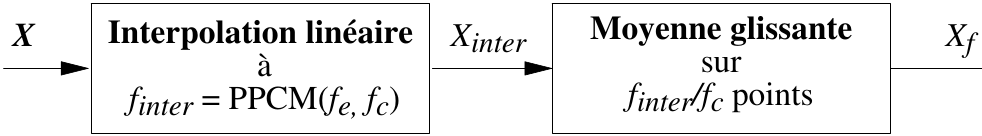
\includegraphics[width=0.8\linewidth]{images/algo_Filtre_moy.png}
\captionof{figure}{Sch�ma fonctionnel de \operfmt{Filtre\_moy}}
\label{fig:algo_Filtre_moy}
}

%%%%%COMMENTAIRE%%%%
\itemstyle{Commentaire~:}
Le passage par PPCM($f_e$, $f_c$) permet de lever l'obligation 
que $f_e$ soit un multiple de $f_c$, mais impose de 
nouvelles conditions :
\begin{itemize}
\item Si $f_c$ est inf�rieure � 1, il peut y avoir des probl�mes
d'arrondi (par ex, 1/15 = 6,666666667e-2, puis ppcm (1/15, 1)=9
au lieu de 1.
\item De fa�on g�n�rale, si PPCM($f_e$, $f_c$) est trop grand, il est
pr\'ef\'erable d'employer une autre technique.
\end{itemize}

%%%%%AUTEUR%%%%
\itemstyle{Auteur~:}
CNRM/GMEI/TRAMM

%%%%%REFERENCE%%%%
\itemstyle{R\'ef\'erences~:}
